\documentclass[12pt]{article}  
% Эта строка — комментарий, она не будет показана в выходном файле  
\usepackage{ucs} 
\usepackage[utf8x]{inputenc} % Включаем поддержку UTF8  
\usepackage[russian]{babel}  % Включаем пакет для поддержки русского языка  
\usepackage{amsmath}
\usepackage{listings}
\usepackage{color}
\usepackage{tikz}
\usepackage{pgfplots}
\usepackage{filecontents}
\usepackage{graphicx}


\definecolor{mygreen}{rgb}{0,0.6,0}
\definecolor{mygray}{rgb}{0.5,0.5,0.5}
\definecolor{mymauve}{rgb}{0.58,0,0.82}
\title{Отчет по лабораторной работе 1 \\ 
	По предмету “Анализ алгоритмов” \\
	По теме “Расстояния Левенштейна и Дамерау-Левенштейна”
}  
\date{2018}  
\author{Фирсова Дарья ИУ7-56}

\begin{document}  
  \maketitle  
  \newpage
\section*{Введение}
В лабораторной работе изучаются расстояние Левенштейна и расстояние Демерау-Левенштейна. Требуется применить метод динамического программирования,  изучить работу алгоритма и получить практические навыки реализации алгоритмов. Задачи для лабораторной работы: 
\begin{enumerate}
\item  Изучение алгоритмов Левенштейна и Дамерау-Левенштейна нахождения расстояния между строками;
\item Применение метода динамического программирования для матричной реализации указанных алгоритмов;
\item Получение практических навыков реализации указанных алгоритмов: двух алгоритмов в матричной версии и одного из алгоритмов в рекурсивной версии;
\item Сравнительный анализ линейной и рекурсивной реализаций выбранного алгоритма определения расстояния между строками по затрачиваемым ресурсам (времени и памяти);
\item Экспериментальное подтверждение различий во временнóй эффективности рекурсивной и нерекурсивной реализаций выбранного алгоритма определения расстояния между строками при помощи разработанного программного обеспечения на материале замеров процессорного времени выполнения реализации на варьирующихся длинах строк;
\item Описание и обоснование полученных результатов в отчете о выполненной лабораторной работе, выполненного как расчётно-пояснительная записка к работе.
\end{enumerate}
\newpage
\section{Аналитическая часть}
Алгоритмы имеют широкое применение: для исправления ошибок в слове при поисковых запросах, вводах текстов и распознавании текстов и речи, для сравнения белков.
\subsection{Описание алгоритмов}
Алгоритм находит редакционное расстояние - последовательность действий, для получения одного слова из другого.
Пусть $S_{1}$  и $S_{2}$ — две строки (длиной $M*M$ и  $N*N$  соответственно) над некоторым алфавитом, тогда редакционное расстояние (расстояние Левенштейна) $d(S_{1},S_{2})$ можно подсчитать по следующей рекуррентной формуле: $d(S_{1},S_{2}) = D(M,N)$ , где $$D(i,j) = \left.
\begin{cases}
	0, & \text  i= 0, j = 0\\
	i, & \text j = 0, i > 0 \\
	j, & \text i = 0, j > 0 \\
	min \begin{cases}
	D(i, j -1) + 1, & \text Insert \\
	D(i-1,j) + 1, & \text  j > 0, i > 0; Delete\\
	D(i -1, j - 1) + m(S_{1}[i],S_{2}[j]) & \text Match\ or \ Replace
	
\end{cases}
\end{cases}
$$
где $m(a,b)$ равна нулю, если $a=b$ единице в противном случае. \\
Для алгоритма Дамерау-Левенштейна существует возможность обмена элемента через один по диагонали.\\
$$d_{a,b}(i,j) = \begin{cases}
\max(i,j) & \text{ if} \min(i,j)=0, \\
\min \begin{cases}
d_{a,b}(i-1,j) + 1 \\
d_{a,b}(i,j-1) + 1 \\
d_{a,b}(i-1,j-1) + 1_{(a_i \neq b_j)} \\
d_{a,b}(i-2,j-2) + 1 
\end{cases} & \text{ if } i,j > 1 \text{ and } a_i = b_{j-1} \text{ and } a_{i-1} = b_j \\
\min \begin{cases}
d_{a,b}(i-1,j) + 1 \\
d_{a,b}(i,j-1) + 1 \\
d_{a,b}(i-1,j-1) + 1_{(a_i \neq b_j)}
\end{cases} & \text{ otherwise,}
\end{cases}
$$
Операция обмена учитывает специфику применения - ошибка в неверном порядке двух букв встречается чаще всего.

\section{Конструкторская часть}
В данном разделе представлены схемы алгоритмов 
\begin{figure}[ht!]
\centering
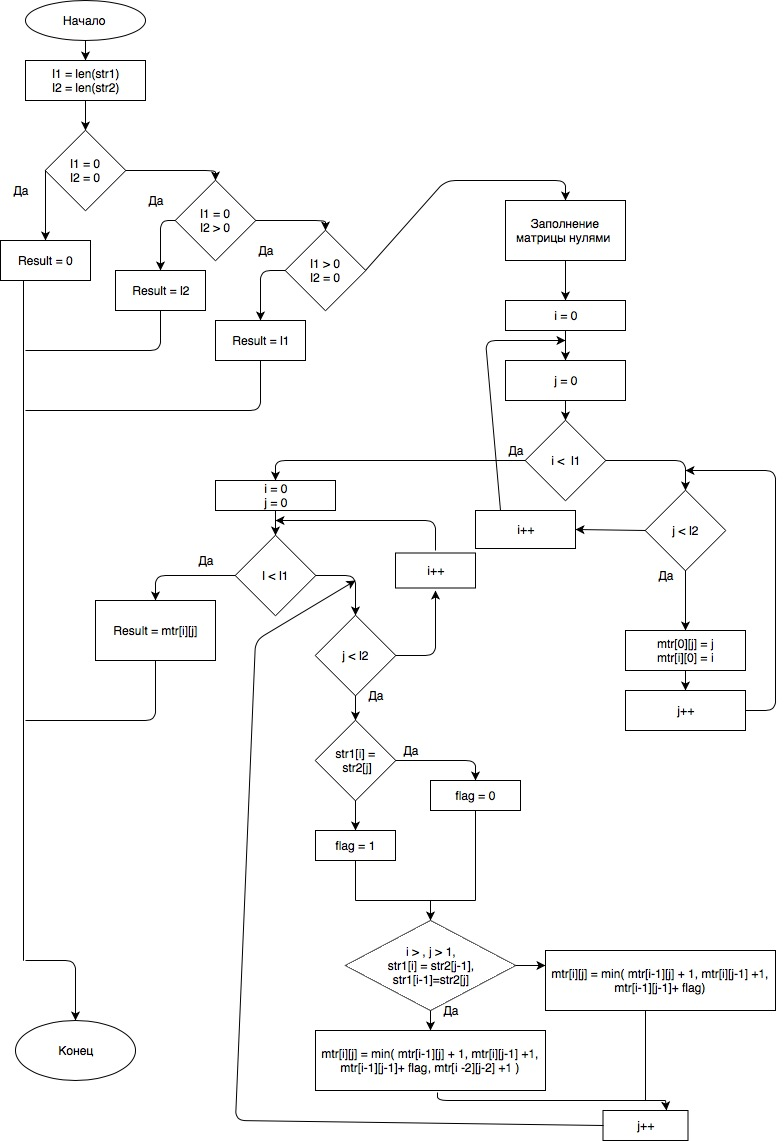
\includegraphics[width=110mm]{damerau.jpg}
\caption{Схема алгоритма Дамерау-Левенштейна \label{overflow}}
\end{figure}


\begin{figure}[ht!]
\centering
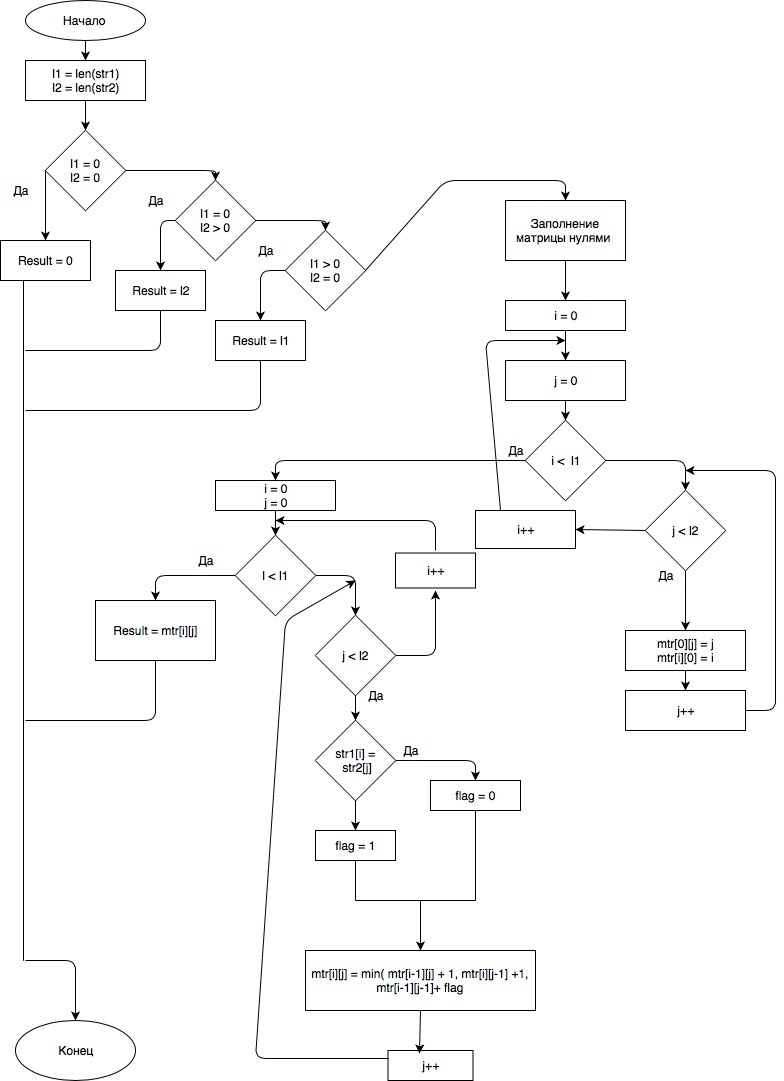
\includegraphics[width=120mm]{levenstein-2.jpg}
\caption{Схема алгоритма Левенштейна  \label{overflow}}
\end{figure}

\newpage
\newpage

\begin{figure}[ht!]
	\centering
	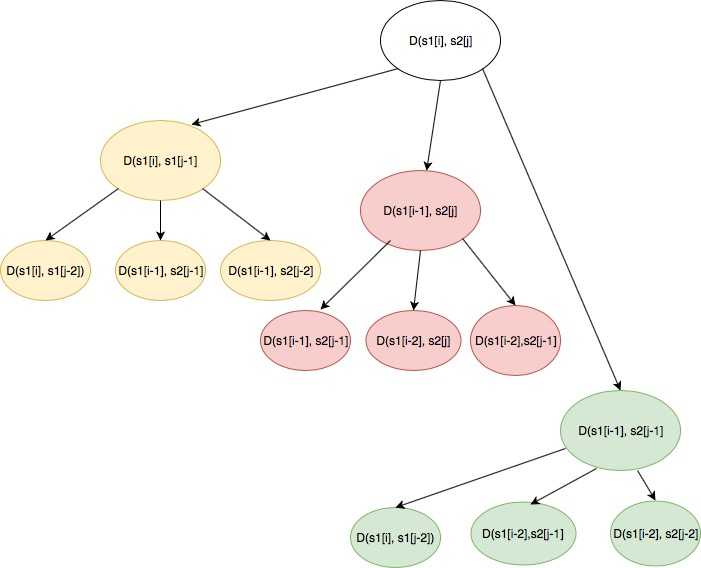
\includegraphics[width=120mm]{list.jpg}
	\caption{Вложенность рекурсии\label{overflow}}
\end{figure}
\begin{figure}[ht!]
	\centering
	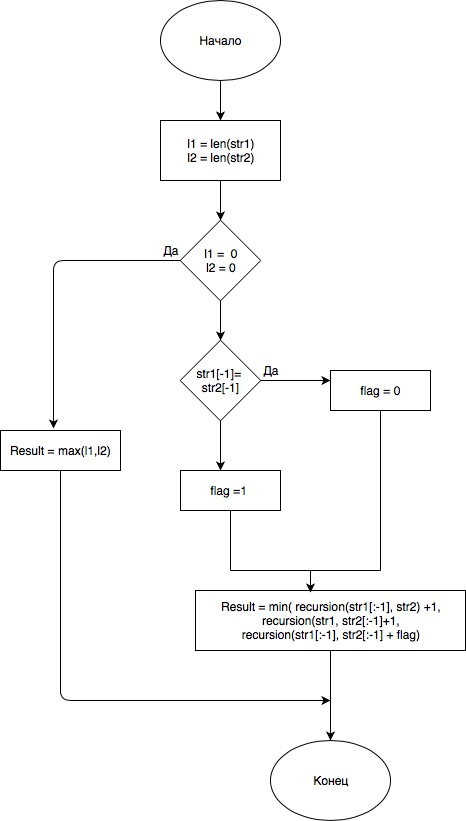
\includegraphics[width=120mm]{recursion.jpg}
	\caption{Схема рекурсивного алгоритма Левенштейна \label{overflow}}
\end{figure}

\newpage
\newpage
\section{Технологическая часть}

В этом разделе приведена реализация функций, указан язык программирования и необходимые модули. 
\subsection{Требования к программному обеспечению}

\subsection{Средства реализации}
В данной работе использовался язык Python 3.6, в среде Pycharm. Для измерения времени использовался модуль time.
\subsection{Листинг кода}
\lstset{ 
	backgroundcolor=\color{white},   % choose the background color; you must add \usepackage{color} or \usepackage{xcolor}; should come as last argument
	basicstyle=\footnotesize,        % the size of the fonts that are used for the code
	breakatwhitespace=false,         % sets if automatic breaks should only happen at whitespace
	breaklines=true,                 % sets automatic line breaking
	captionpos=b,                    % sets the caption-position to bottom
	commentstyle=\color{mygreen},    % comment style
	deletekeywords={...},            % if you want to delete keywords from the given language
	escapeinside={\%*}{*)},          % if you want to add LaTeX within your code
	extendedchars=true,              % lets you use non-ASCII characters; for 8-bits encodings only, does not work with UTF-8
	frame=single,	                   % adds a frame around the code
	keepspaces=true,                 % keeps spaces in text, useful for keeping indentation of code (possibly needs columns=flexible)
	keywordstyle=\color{blue},       % keyword style
	language=Python,                 % the language of the code
	morekeywords={*,...},            % if you want to add more keywords to the set
	numbers=left,                    % where to put the line-numbers; possible values are (none, left, right)
	numbersep=5pt,                   % how far the line-numbers are from the code
	numberstyle=\tiny\color{mygray}, % the style that is used for the line-numbers
	rulecolor=\color{black},         % if not set, the frame-color may be changed on line-breaks within not-black text (e.g. comments (green here))
	showspaces=false,                % show spaces everywhere adding particular underscores; it overrides 'showstringspaces'
	showstringspaces=false,          % underline spaces within strings only
	showtabs=false,                  % show tabs within strings adding particular underscores
	stepnumber=1,                    % the step between two line-numbers. If it's 1, each line will be numbered
	stringstyle=\color{mymauve},     % string literal style
	tabsize=2,	                   % sets default tabsize to 2 spaces
	title=\lstname                   % show the filename of files included with \lstinputlisting; also try caption instead of title
}
\lstinputlisting[language=Python]{functions.py}
\newpage
\section{Экспериментальная часть}
В данном разделе будут приведены примеры работы программы для трех разных вариантов: стандартный алгоритм Левенштейна, алгоритм Дамерау-Левенштейна, и рекурсивный алгоритм Левенштейна. Приведет сравнительный анализ двух нерекурсивных алгоритмов при тестах от 100 до 1100 букв в слове. Тесты всех трех алгорит
\subsection{Примеры работы}
\begin{center}
	\begin{tabular}{| l | l | l | l |}
		\hline
		Входные данные & Левенштейн & Дамерау & Рекурсия \\ \hline
		aaba, abab & 2 & 2 & 2 \\ \hline
		qwerty , wqeryt & 4 & 2 & 4 \\ \hline
		polynomial, exponential & 6 & 6 & 6 \\ \hline
		tartar, otara & 3 & 3 & 3 \\ \hline
		\hline
	\end{tabular}
\newline
Пример результата работы матричной реализации для тестовых данных polynom, exponent
\newline
$$\begin{vmatrix} 
0 & 1 & 2 & 3 & 4 & 5 & 6 & 7 \\
1 & 1 & 2 & 3 & 4 & 5 & 6 & 7 \\ 
2 & 2 & 2 & 3 & 4 & 5 & 6 & 7 \\ 
3 & 2 & 3 & 3 & 4 & 5 & 6 & 7 \\ 
4 & 3 & 2 & 3 & 4 & 5 & 5 & 6 \\ 
5 & 4 & 3 & 3 & 4 & 4 & 5 & 6 \\ 
6 & 5 & 4 & 4 & 4 & 5 & 5 & 6 \\ 
7 & 6 & 5 & 5 & 5 & 4 & 5 & 6 \\ 
8 & 7 & 6 & 6 & 6 & 5 & 5 & 6 \\
\end{vmatrix}$$
\end{center}
\subsection{Сравнительный анализ}
Сравнение алгоритма Левенштейна  и Дамерау-Левенштейна
\newline
\begin{tikzpicture}
\begin{axis}
[
	axis x line=middle,
	axis y line=middle,
	enlarge y limits=true,
	xmin=0, xmax=1100,
	ymin=0, ymax=1500,
	width=15cm, height=15cm,     % size of the image
	grid = major,
	grid style={dashed, gray!30},
	ylabel=Время,
	xlabel=Длина,
	legend style={at={(0.1,-0.1)}, anchor=north}
]
\addplot table [x=length, y=basic, col sep=comma] {output.txt};
\addplot table [x=length, y=damerau, col sep=comma] {output.txt};
\end{axis}
\end{tikzpicture}
\newpage
Сравнение с рекурсией\\
\begin{tikzpicture}
\begin{axis}
[
axis x line=middle,
axis y line=middle,
enlarge y limits=true,
xmin=3, xmax=11,
ymin=0, ymax=9000,
width=15cm, height=15cm,     % size of the image
grid = major,
grid style={dashed, gray!30},
ylabel=Время,
xlabel=Длина,
legend style={at={(0.1,-0.1)}, anchor=north}
]
\addplot table [x=length, y=basic, col sep=comma] {rec.txt};
\addplot table [x=length, y=damerau, col sep=comma] {rec.txt};
\addplot table [x=length, y=recursion, col sep=comma] {rec.txt};
\end{axis}
\end{tikzpicture}
\section{Вывод}
В ходе лабораторной работы были проанализированы алгоритмы поиска редакционного расстояния. Приведена практическая реализация алгоритмов. Для составления отчета был изучен язык разметки и математических фунцкий Latex.
\end{document}